%%%%%%%%%%%%%%%%%%%%%%%%%%%%%%%%%%%
% math and Students
%%%%%%%%%%%%%%%%%%%%%%%%%%%%%%%%%%%
\section{Math and Students}
Now that it has been established that teachers struggle with large classes, it is relevant to investigate the issues that students have, which will be done in the context of math. This section will set out to explore the relationship between math, one of the most important areas of study, and the students of today, as well as to if, how and why that relationship can be improved upon.

%%%%%%%%%%%%%%%%%%%%%%%%%%%%%
% What is Math?
%%%%%%%%%%%%%%%%%%%%%%%%%%%%%
\subsection{What is Math?}
Math is one of the most important subjects studied in schools today. Math is an area of study that deals with logic and reasoning around quantity, shape and arrangement \cite{HomWhatMathematics}. 
\newline\indent
The human ability to comprehend numbers and perform calculations is what civilization is built upon \cite{RomanMathImportance}. Math is so ingrained into human society that its influence on our world is hard to grasp. Not only is math a crucial element in the functioning of our world, when learning math one must make use of and improve many critical cognitive functions \cite{CognitiveEdCircuit}. The massive importance of math and cognitive benefits the learning of it provides is why it is a subject taught throughout the world and in all levels of education.
\newline\newline
In the Danish educational system, math is a mandatory subject through primary and lower secondary education \cite{SubjectsEducation}, and in secondary education math is split into three levels, C, B and A \cite{StxUndervisningsministeriet}, where C level is the lowest level of math and A is the highest. C level math covers the essential knowledge required to perform math and is the basis for learning B and A level math \cite{2017Matematik-C-stx-august-2017}. 
 
%%%%%%%%%%%%%%%%%%%%%%%%%%%%%
% Is Math Difficult?
%%%%%%%%%%%%%%%%%%%%%%%%%%%%%
\subsection{Is Math Difficult?}

Since math is so important, it is evident that our ability to perform math is crucial. As such math has been at the forefront of human study, and our ability to comprehend and make use of it has developed with time. Why is it then, that math is one of the subjects that students struggle with the most?
\newline\newline
The results of the May 2018 statistical bulletin for the Diploma Programme of the \newacr{International Baccalaureate}{IB}, an international educational foundation respected across the globe \cite{WhatBaccalaureate}, show that the mean grade out of their 7-point system for students in the two lowest levels of the compulsive mathematical studies (and the two largest) were often significantly lower than the mean grades in the individuals and societies studies \cite{Baccalaureate2018TheSession}. \Figureref{fig:grade_distribution} shows the results for maths and a selection of languages, of which the A level English courses are also a part of. It is important to note that English is also a mandatory subject in the IB. It's \newacr{Standard Level}{SL}, just like math, contains the results of students that chose to study it at the lowest level, making it's results less skewed towards a higher mean grade based on the virtue of it's students not having some affinity or preference towards the subject. It is clear to see that the mean grade for SL of both English A \newacr{Language and Literature}{LAL} and \newacr{Literature}{LIT} are significantly higher than that of SL Math Studies Mathematics. One can also see that out of the Math Standard Level and Math Studies courses, which combined encompass over 80,000 students, roughly 30\% received a grade below 4 on the 7-point system. In comparison, in English A LAL and LIT roughly less than 5\% of students recived a grade less than 4. In fact all other courses frequently only have 15-25\% scoring below a 4 on the 7-point system. The mean grades in the sciences, most of which make large use of math, were also lower than those in the individuals and societies. This trend can be seen in all of their available statistics bulletins for their Diploma Programme, spanning from November 2005 to May 2018, as well as in their Middle Years Programme. It is clear from analyzing the statistics from the IB that students struggle to perform more in math and subjects that make use of it than any other subject.

\begin{figure}[H]
\centering
    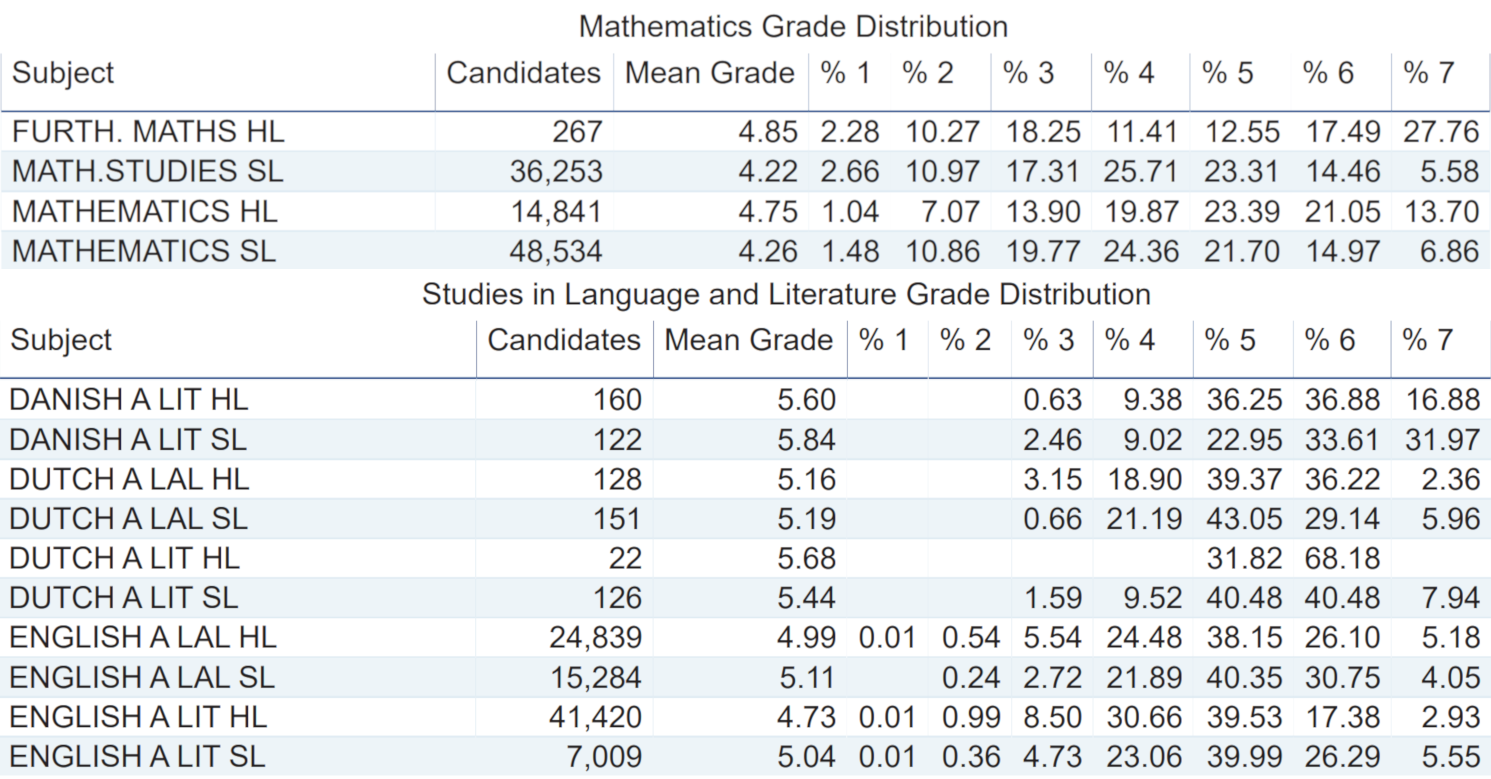
\includegraphics[width=0.85\textwidth]{figures/grade_distribution.png}
    \caption{Grade Distribution in Math and a couple of Languages and Literature Studies \cite{Baccalaureate2018TheSession}}
    \label{fig:grade_distribution}
\end{figure}

\noindent
A poll from gallup.com, a large management consulting company known for for its public opinion polls, asked U.S students between the ages of 13 and 17 which subjects they found most difficult in school, and math came out on top \cite{MathTeens}. This shows that the results provided by the IB's statistical bulletins are not just the results of specific grading techniques or boundaries, but because a portion of students do struggle with it. The Gallup poll also shows that the percentage of students that said they found math difficult was between 30\% to 40\%. 
\newline\newline
These two sources paint a picture that math is indeed a subject that seems to be challenging. It is apparent in both the results and opinions of students who study math. Denmark is no exception to these trends \cite{JessenMatematikudredningen}. 

%%%%%%%%%%%%%%%%%%%%%%%%%%%%%
% Why is Math Difficult?
%%%%%%%%%%%%%%%%%%%%%%%%%%%%%
\subsection{Why is Math Difficult?} 
\label{sub:why_is_math_difficult}
The next leap is to ask why it is so. Why is it that students could have issues with an area of study that has been integral to the development of our world? Some point the finger at a concept known as \enquote{math anxiety} \cite{BeilockSianMathIt}. Math anxiety is what it's name would imply, a feeling of tension, apprehension, or fear that interferes with math performance \cite{Ashcraft2002MathConsequences}.
\newline\newline
Math anxiety is a concept that has only more recently been brought into the limelight. Research into the subject only kicked off in the 1970s, which is significant given that math has been an integral part of human society for millennia. Since then, many reports and articles have been published that focused on the relationships between math anxiety and other characteristics. 
\newline\newline
The Hembree meta-analysis is one of the most well know reports regarding math anxiety \cite{Hembree1990THEANXIETY}. According to the findings of this report, the higher one’s math anxiety, the lower one’s ability  towards learning, mastery, and motivation in regards to math is. highly math-anxious individuals get poorer grades in the math classes they take, show low motivation to take more math, and in fact do take less math. they clearly learn less math than their low-anxious counterparts. Simply put, as math anxiety increases, math achievement declines. Math anxiety is also not exclusive to a small percentage of students. One study found that up to 50\% of students in English secondary schools suffer from some level of math anxiety \cite{NormanMathsStudents}.  
\newline\newline
It has also been theorized that math anxiety starts in the classroom. It has been found that the approach the teacher has to teaching can severely affect the ability of the students learn, and can create the perfect environment for math anxiety to develop. It has actually been shown that  lower-than-average math abilities and/or working memory capacity, susceptibility to public embarrassment, and a non supportive teacher all may be risk factors for developing math anxiety \cite{Ashcraft2002MathConsequences}.
\newline\newline
It is easy to imagine how math anxiety affects learning, say in a high school math classroom. A student with math anxiety diverts attention away from the content of the class and toward internal worries and anxieties over math. This can only slow or degrade the mastery of the to-be-learned information. 
\newline\newline
Math anxiety is exclusive to math, there are other elements that interfere with learning as a whole. Disabilities that effect learning, such as Dyslexia, Dysgraphia and Dyscalculia, or related disorders, such as ADHD, are also elements that can affect one's ability to understand math\cite{TypesDisabilities}. However, There are many different learning disabilities and disorders, which in turn leads to a massive variety in their effects on learning as well as the strategies one must employ to counter them. Focusing on explaining how math anxiety affects learning bears greater importance than trying to do the same with even the most common learning disabilities and disorders, as it is exclusive to the subject this report is focused upon and is more common than any individual learning disability. 
\newline \newline
Although it is important to be aware of math anxiety, and to a lesser extent learning disabilities, this report will however cater towards the learning process as a whole, as it encompasses all students as well as teachers. 